\chapter{Conclusion}

This chapter describes the final state of the XOXOmail application, as well as suggestions for further development of the application. The chapter starts off with section \ref{con_sys_over} that describes how the XOXOmail looked and behaved when the implementation was finished. Section \ref{con_testing} lists and discusses the final tests results, as well as describes what improvements we made from the usability testing results. Section \ref{con_further} discusses the possible ways one could improve and extend the application. Section \ref{con_fullfill} details how we have fullfilled the different functional and non-functional requirements. Section \ref{con_summary} contains a conclusion of this chapter.

\section{System overview}\label{con_sys_over}
This section will give an overview of the XOXOmail application after the implementation ended. It starts of by discussing the architecture, continues to discussing the user interface of the application and concludes with discussion the combined functionality of the application.

\subsection{Architecture}
The final architecture is very much like the planned architecture and the full description of the architecture can be found in chapter \ref{chapter_architecture}.

\subsection{Graphical user interface}
The final version of the graphical user inteface is described here by showing the most important screens from the application, as well as the reason behind the most important choices made. The evolution of the user interface during the different sprints is documented in the sprint chapters.

\paragraph{The tab navigation system}\hfill
\newline
The choice of a main form of navigation fell on a tabbed system, as seen in figure \ref{fig:frontend_inbox} on page \pageref{fig:frontend_inbox}. The initial thought behind using this form of navigation was that we got an easy way of navigating around the different views and a quick view of the available views.
At a later point we figured out that the tab navigation is supposed to be used for switching between different views of the same type, which is not the case in our application. We also ran into some problems with the built-in Android tab component. Unfortunately this was at a point too late to conduct any drastical changes, and we think that the solution is well enough suited for this prototype.

\begin{figure}[H]
\begin{center}
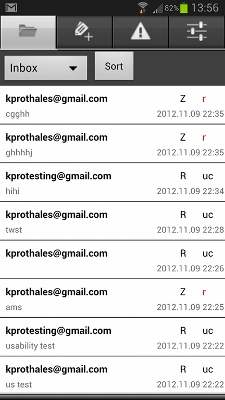
\includegraphics{inbox_final}
\end{center}
\caption{Inbox screen view} \label{fig:frontend_inbox}
\end{figure}

\paragraph{The inbox}\hfill
\newline
The inbox folder and sent messages folder are composed in an identical way. We used a list where we specified a custom layout of each message item in the list, as seen in figure \ref{fig:frontend_inbox} on page \pageref{fig:frontend_inbox}. All the information on each item was requested by Thales, and we tried to make it look like a the standard way of listing mails 
in an inbox. We used abbreviations for the security labels (e.g. the Z and R) and priorities (e.g. r and uc) as specified by Thales because of the limited space of each message item. We also added the common clip icon to inform the user that the message has files attached. 

\newpage

\paragraph{Messages}\hfill
\newline
If the user clicks an item in the message list he is sent to the view for showing the full information of the message, as seen in figure \ref{fig:frontend_message} on page \pageref{fig:frontend_message}. We chose to list the military messaging attributes in a separate box to easy give an overview of them. We originally had a more elaborate plan as to show the attachments, but ended up with a button the opens a dialog box as this was easier to implement, and we were short on time. 
%We originally planned to have a fancy function that showed the attachments, but ended up with a button that opens a dialog box as this was easier to implement and was created towards the end of the %project. 
The common choices of replying to and forwarding a message, as well as buttons with arrows to browse between the messages are placed at the bottom of the screen.

\begin{figure}[h!]
\begin{center}
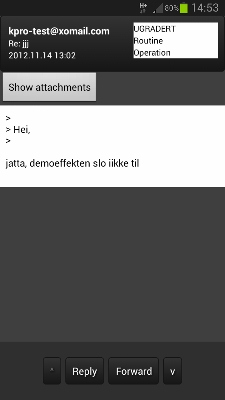
\includegraphics{message_final}
\end{center}
\caption{Message screen view} \label{fig:frontend_message}
\end{figure}

\newpage

\paragraph{Sending a message}\hfill 
\newline
The view for sending messages is broken down into the logical part of a message conforming to the \gls{mmhs} standards, as shown in figure \ref{fig:frontend_messagesend} on page \pageref{fig:frontend_messagesend}.
%The view for sending a message is composed of what we think is the logical way of entering the information, as shown in figure \ref{fig:frontend_messagesend} on page \pageref{fig:frontend_messagesend}.
The selection of military attributes are realized by the use of the Android component spinner, which from a behavioural aspect looks like a drop-down menu.
%We used the same way of selecting the military attributes, namely to use what Android calls a spinner, a kind of a drop-down list with all the available attributes. 
As the diligent reader may have noticed, there is no button for sending the message. This is however just because view is bigger then the screen, and scrolling down to the bottom of the view would reveal the button. 
%Though the button for sending is not visible in the screenshot, because the screen is scrollable.

\begin{figure}[h!]
\begin{center}
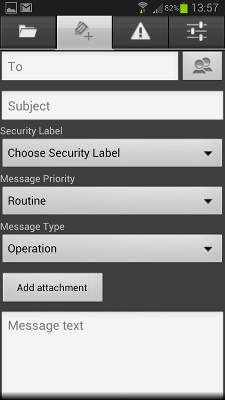
\includegraphics{sendmessage_final}
\end{center}
\caption{Sending message screen view} \label{fig:frontend_messagesend}
\end{figure}

\newpage

\paragraph{Instant message}\hfill
\newline
The requirement for instant messages was that it should be possible to send an instant message by using three or less user actions. We thought about different ways of doing this, but ended up with the solution that is shown in figure \ref{fig:frontend_instamessage} on page \pageref{fig:frontend_instamessage}.
One has to set the standard attributes for the instant message in the settings, thus requiring a couple of actions before being able to send an instant message, but after this step one can send instant messages with no more than three clicks (e.g. push the instant message tab, enter text and push send). 

\begin{figure}[H]
\begin{center}
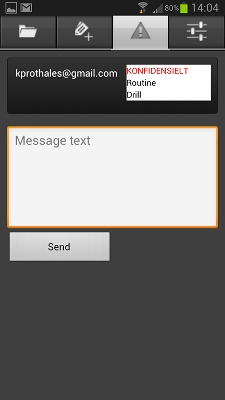
\includegraphics{instantmessage_final}
\end{center}
\caption{Sending instant message screen view} \label{fig:frontend_instamessage}
\end{figure}

\subsection{Functionality}
The XOXOmail application has a quite extensive functionality, although we did not manage to implement all functional requirements.
The functional requirements that were not implemented or finished are listed below:
\begin{itemize}
\item{}Address book - partly implemented (FR5)
\item{}Video attachments - not implemented (parts of FR7)
\item{}Delete message - partly implemented (parts of FR8)
\item{}Message status - not implemented (FR11)
\item{}Search - not implemented (FR14)
\item{}Signing of messages - partly implemented (FR15)
\end{itemize}